\chapter{Discussão dos Resultados}

Para avaliarmos a qualidade dos modelos, utilizamos as seguintes métricas: 

\begin{itemize}
    \item Acurácia do produtor (precisão): de todos os elementos de uma classe, quantos por cento, o modelo conseguiu identificar; 
    \item Acurácia do usuário (revocação): de todos os elementos que o modelo identificou como uma determinada classe, quantos por cento, são realmente daquela classe; 
    \item \textit{F1-Score}: é a média harmônica da acurácia do produtor e do usuário. É calculado utilizando a formulá: $\frac{2 * AP * AU}{AP + AU}$, onde AP é a acurácia do produtor e AU é a acurácia do usuário.
\end{itemize}

Na Figura \ref{fig:analise_acuracia}, apresentamos o resultado da análise de acurácia utilizando o conjunto de dados de teste para os três modelos desenvolvidos. Avaliando os resultados, é possível constatarmos que, entre os dois modelos baseados em \textit{Random Forest}, o modelo sem o balanceamento das classes atingiu melhores resultados do que o modelo com balanceamento das classes. Já entre os três modelos desenvolvidos, o modelo baseado em LSTM, que utiliza o contexto de toda a série temporal para a classificação, atingiu os melhores resultados. 

\begin{figure}[H]
\caption{Matrizes de confusão com a análise de acurácia para os modelos: a) \textit{Random Forest} sem balanceamento das classes, b) \textit{Random Forest} com balanceamento das classes e c) modelo baseado na LSTM.}
\label{fig:analise_acuracia}
\centering
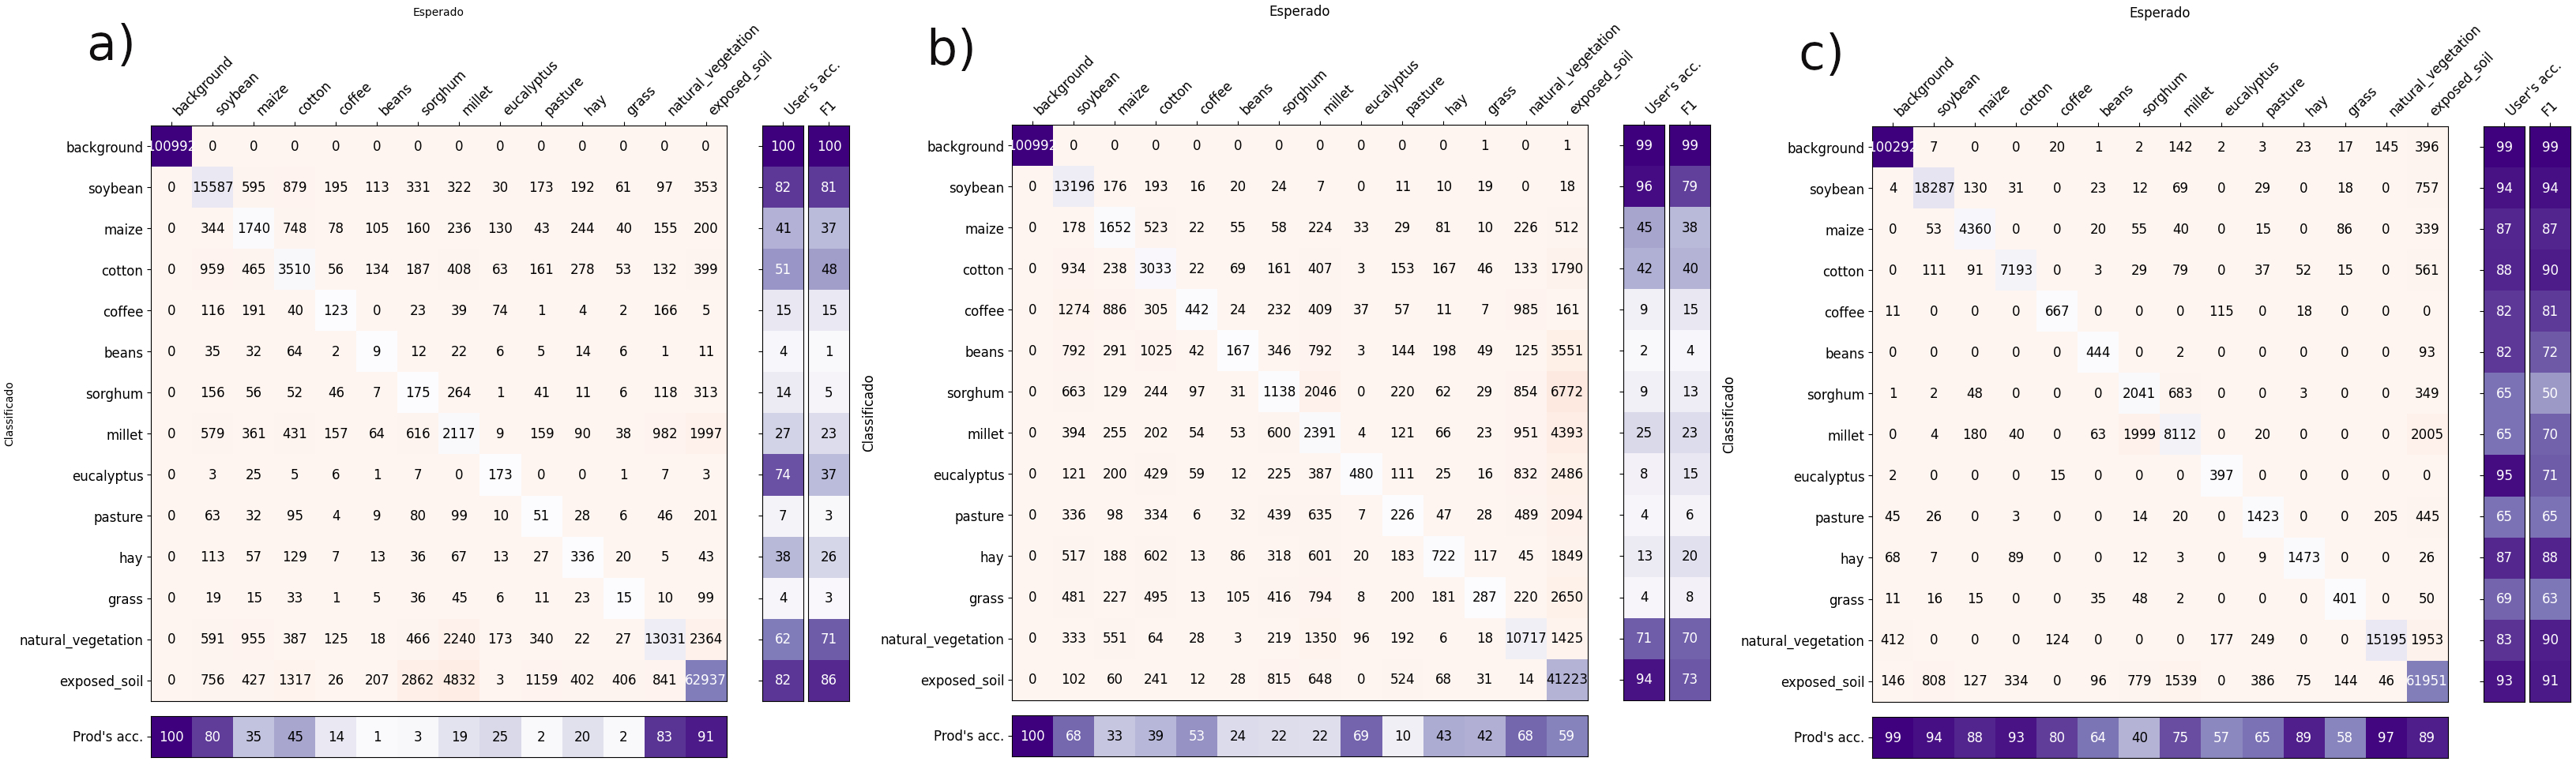
\includegraphics[width=\textwidth]{figuras/analise_acuracia.jpg}
\end{figure}

Após avaliarmos a acurácia dos resultados, utilizamos o modelo baseado em LSTM, que alcançou os melhores resultados, para gerarmos mapas de uso e cobertura da terra para o período de 01/10/2020 à 30/09/2021 em um recorte da mesorregião do Extremo Oeste Baiano, Bahia (Figura \ref{fig:serie_temporal_resultado}). 

\begin{figure}[H]
\caption{Resultado da classificação do uso e cobertura da terra para o período de 01/10/2020 à 30/09/2021 em um recorte da mesorregião do Extremo Oeste Baiano, Bahia. }
\label{fig:serie_temporal_resultado}
\centering
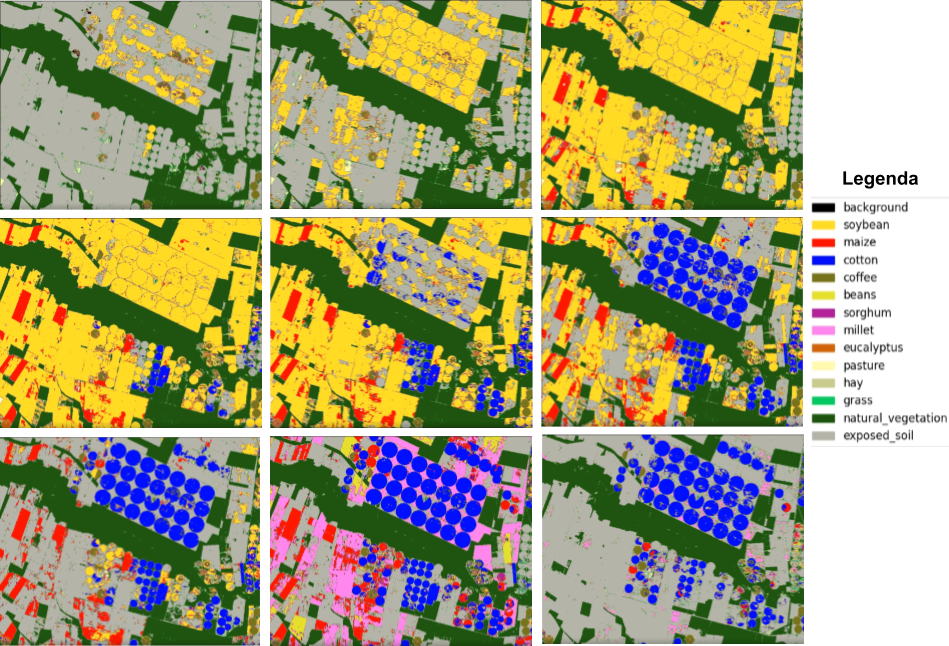
\includegraphics[width=0.8\textwidth]{figuras/serie_temporal_resultado.png}
\begin{tablenotes}
\item Vídeo completo disponível em: \url{https://www.youtube.com/watch?v=R6SwGzosLfM}.
\end{tablenotes}
\end{figure}

Na Figura \ref{fig:serie_temporal_resultado}, é possível observarmos o momento em que os talhões ainda estão com solo exposto, em seguida os talhões de soja e milho são plantados, permanecem por algum tempo em campo, e logo depois são colhidos, dando lugar à talhões de algodão e milhete, que também são colhidos e voltam a ficar com o solo exposto. 


\renewcommand{\cleardoublepage}{}
\renewcommand{\clearpage}{}
\vspace{5mm}